% Options for packages loaded elsewhere
% Options for packages loaded elsewhere
\PassOptionsToPackage{unicode}{hyperref}
\PassOptionsToPackage{hyphens}{url}
\PassOptionsToPackage{dvipsnames,svgnames,x11names}{xcolor}
%
\documentclass[
]{article}
\usepackage{xcolor}
\usepackage{amsmath,amssymb}
\setcounter{secnumdepth}{5}
\usepackage{iftex}
\ifPDFTeX
  \usepackage[T1]{fontenc}
  \usepackage[utf8]{inputenc}
  \usepackage{textcomp} % provide euro and other symbols
\else % if luatex or xetex
  \usepackage{unicode-math} % this also loads fontspec
  \defaultfontfeatures{Scale=MatchLowercase}
  \defaultfontfeatures[\rmfamily]{Ligatures=TeX,Scale=1}
\fi
\usepackage{lmodern}
\ifPDFTeX\else
  % xetex/luatex font selection
\fi
% Use upquote if available, for straight quotes in verbatim environments
\IfFileExists{upquote.sty}{\usepackage{upquote}}{}
\IfFileExists{microtype.sty}{% use microtype if available
  \usepackage[]{microtype}
  \UseMicrotypeSet[protrusion]{basicmath} % disable protrusion for tt fonts
}{}
\makeatletter
\@ifundefined{KOMAClassName}{% if non-KOMA class
  \IfFileExists{parskip.sty}{%
    \usepackage{parskip}
  }{% else
    \setlength{\parindent}{0pt}
    \setlength{\parskip}{6pt plus 2pt minus 1pt}}
}{% if KOMA class
  \KOMAoptions{parskip=half}}
\makeatother
% Make \paragraph and \subparagraph free-standing
\makeatletter
\ifx\paragraph\undefined\else
  \let\oldparagraph\paragraph
  \renewcommand{\paragraph}{
    \@ifstar
      \xxxParagraphStar
      \xxxParagraphNoStar
  }
  \newcommand{\xxxParagraphStar}[1]{\oldparagraph*{#1}\mbox{}}
  \newcommand{\xxxParagraphNoStar}[1]{\oldparagraph{#1}\mbox{}}
\fi
\ifx\subparagraph\undefined\else
  \let\oldsubparagraph\subparagraph
  \renewcommand{\subparagraph}{
    \@ifstar
      \xxxSubParagraphStar
      \xxxSubParagraphNoStar
  }
  \newcommand{\xxxSubParagraphStar}[1]{\oldsubparagraph*{#1}\mbox{}}
  \newcommand{\xxxSubParagraphNoStar}[1]{\oldsubparagraph{#1}\mbox{}}
\fi
\makeatother


\usepackage{longtable,booktabs,array}
\usepackage{calc} % for calculating minipage widths
% Correct order of tables after \paragraph or \subparagraph
\usepackage{etoolbox}
\makeatletter
\patchcmd\longtable{\par}{\if@noskipsec\mbox{}\fi\par}{}{}
\makeatother
% Allow footnotes in longtable head/foot
\IfFileExists{footnotehyper.sty}{\usepackage{footnotehyper}}{\usepackage{footnote}}
\makesavenoteenv{longtable}
\usepackage{graphicx}
\makeatletter
\newsavebox\pandoc@box
\newcommand*\pandocbounded[1]{% scales image to fit in text height/width
  \sbox\pandoc@box{#1}%
  \Gscale@div\@tempa{\textheight}{\dimexpr\ht\pandoc@box+\dp\pandoc@box\relax}%
  \Gscale@div\@tempb{\linewidth}{\wd\pandoc@box}%
  \ifdim\@tempb\p@<\@tempa\p@\let\@tempa\@tempb\fi% select the smaller of both
  \ifdim\@tempa\p@<\p@\scalebox{\@tempa}{\usebox\pandoc@box}%
  \else\usebox{\pandoc@box}%
  \fi%
}
% Set default figure placement to htbp
\def\fps@figure{htbp}
\makeatother


% definitions for citeproc citations
\NewDocumentCommand\citeproctext{}{}
\NewDocumentCommand\citeproc{mm}{%
  \begingroup\def\citeproctext{#2}\cite{#1}\endgroup}
\makeatletter
 % allow citations to break across lines
 \let\@cite@ofmt\@firstofone
 % avoid brackets around text for \cite:
 \def\@biblabel#1{}
 \def\@cite#1#2{{#1\if@tempswa , #2\fi}}
\makeatother
\newlength{\cslhangindent}
\setlength{\cslhangindent}{1.5em}
\newlength{\csllabelwidth}
\setlength{\csllabelwidth}{3em}
\newenvironment{CSLReferences}[2] % #1 hanging-indent, #2 entry-spacing
 {\begin{list}{}{%
  \setlength{\itemindent}{0pt}
  \setlength{\leftmargin}{0pt}
  \setlength{\parsep}{0pt}
  % turn on hanging indent if param 1 is 1
  \ifodd #1
   \setlength{\leftmargin}{\cslhangindent}
   \setlength{\itemindent}{-1\cslhangindent}
  \fi
  % set entry spacing
  \setlength{\itemsep}{#2\baselineskip}}}
 {\end{list}}
\usepackage{calc}
\newcommand{\CSLBlock}[1]{\hfill\break\parbox[t]{\linewidth}{\strut\ignorespaces#1\strut}}
\newcommand{\CSLLeftMargin}[1]{\parbox[t]{\csllabelwidth}{\strut#1\strut}}
\newcommand{\CSLRightInline}[1]{\parbox[t]{\linewidth - \csllabelwidth}{\strut#1\strut}}
\newcommand{\CSLIndent}[1]{\hspace{\cslhangindent}#1}



\setlength{\emergencystretch}{3em} % prevent overfull lines

\providecommand{\tightlist}{%
  \setlength{\itemsep}{0pt}\setlength{\parskip}{0pt}}



 


\usepackage{booktabs}
\usepackage{longtable}
\usepackage{array}
\usepackage{multirow}
\usepackage{wrapfig}
\usepackage{float}
\usepackage{colortbl}
\usepackage{pdflscape}
\usepackage{tabu}
\usepackage{threeparttable}
\usepackage{threeparttablex}
\usepackage[normalem]{ulem}
\usepackage{makecell}
\usepackage{xcolor}
\usepackage{siunitx}

    \newcolumntype{d}{S[
      table-align-text-before=false,
      table-align-text-after=false,
      input-symbols={-,\*+()}
    ]}
  
\usepackage{float}
\usepackage{array}
% reset numbering after abstract
\usepackage{etoolbox}
\AtBeginEnvironment{abstract}{\setcounter{section}{0}}
% Custom table row spacing
\renewcommand{\arraystretch}{0.9}
\makeatletter
\@ifpackageloaded{caption}{}{\usepackage{caption}}
\AtBeginDocument{%
\ifdefined\contentsname
  \renewcommand*\contentsname{Table of contents}
\else
  \newcommand\contentsname{Table of contents}
\fi
\ifdefined\listfigurename
  \renewcommand*\listfigurename{List of Figures}
\else
  \newcommand\listfigurename{List of Figures}
\fi
\ifdefined\listtablename
  \renewcommand*\listtablename{List of Tables}
\else
  \newcommand\listtablename{List of Tables}
\fi
\ifdefined\figurename
  \renewcommand*\figurename{Figure}
\else
  \newcommand\figurename{Figure}
\fi
\ifdefined\tablename
  \renewcommand*\tablename{Table}
\else
  \newcommand\tablename{Table}
\fi
}
\@ifpackageloaded{float}{}{\usepackage{float}}
\floatstyle{ruled}
\@ifundefined{c@chapter}{\newfloat{codelisting}{h}{lop}}{\newfloat{codelisting}{h}{lop}[chapter]}
\floatname{codelisting}{Listing}
\newcommand*\listoflistings{\listof{codelisting}{List of Listings}}
\makeatother
\makeatletter
\makeatother
\makeatletter
\@ifpackageloaded{caption}{}{\usepackage{caption}}
\@ifpackageloaded{subcaption}{}{\usepackage{subcaption}}
\makeatother
\usepackage{bookmark}
\IfFileExists{xurl.sty}{\usepackage{xurl}}{} % add URL line breaks if available
\urlstyle{same}
\hypersetup{
  pdftitle={Local Heterogeneity in Artificial Intelligence Jobs Over Time and Space},
  pdfauthor={Jacob Khaykin; David Kane},
  colorlinks=true,
  linkcolor={blue},
  filecolor={Maroon},
  citecolor={Blue},
  urlcolor={Blue},
  pdfcreator={LaTeX via pandoc}}


\title{Local Heterogeneity in Artificial Intelligence Jobs Over Time and
Space}
\usepackage{etoolbox}
\makeatletter
\providecommand{\subtitle}[1]{% add subtitle to \maketitle
  \apptocmd{\@title}{\par {\large #1 \par}}{}{}
}
\makeatother
\subtitle{A Replication Study of Andreadis et al.~(AEA Papers and
Proceedings, 2025)}
\author{Jacob Khaykin\footnote{Solon High School,
  \href{mailto:jacobkhaykin27@solonschools.net}{\nolinkurl{jacobkhaykin27@solonschools.net}}} \and David
Kane\footnote{New College of Florida,
  \href{mailto:dakane@ncf.edu}{\nolinkurl{dakane@ncf.edu}}}}
\date{}
\begin{document}
\maketitle


\emph{JEL: J24, O33, R11}

\emph{Keywords:} Artificial Intelligence, Regional Economics, Labor
Markets

\emph{Data Availability:} The R code and data to reproduce this
replication are available in this repository:
https://github.com/JacobKhay/Andreadis-Replication.

\section*{Abstract}\label{abstract}
\addcontentsline{toc}{section}{Abstract}

We replicate Andreadis et al. (\citeproc{ref-andreadis2025}{2025}) on
the correlation between the level and growth of artificial intelligence
employment and education, innovation, and industry factors across U.S.
counties from 2014 to 2023. We successfully reproduce their main results
and extend the analysis by employing log-population weights to assess
robustness. The core associations persist, though almost all magnitudes
shrink. We also highlight unsupported causal claims in Andreadis et al.
(\citeproc{ref-andreadis2025}{2025}), given its observational design.

Declaration: There are no financial conflicts of interest to share.

\newpage

\section{Introduction}\label{introduction}

This paper replicates the analysis of Andreadis et al.
(\citeproc{ref-andreadis2025}{2025}) on the correlation between the
level and growth artificial intelligence employment openings and
education, innovation, and industry factors across U.S. counties from
2014 to 2023. Understanding where AI employment emerges and how it
spreads is important for both researchers and policymakers, since the
rise of AI has the potential to reshape regional economies
(\citeproc{ref-acemoglu2024}{Acemoglu, 2024};
\citeproc{ref-brynjolfsson2021}{Brynjolfsson, Rock, and Syverson,
2021}), alter the demand for skills
(\citeproc{ref-acemoglu2019}{Acemoglu and Restrepo, 2019};
\citeproc{ref-autor2015}{Autor, 2015}), and shift patterns of innovation
(\citeproc{ref-babina2024}{Babina et al., 2024}). County-level variation
offers a granular perspective on how these transformations take hold
across the United States.

The outcome of interest is the share of AI-related job postings at the
county-year level. This measure captures both the absolute level of AI
employment opportunities and how those opportunities evolve over time.
Tracking these dynamics provides insight into which regions gain early
access to AI-driven growth and which lag behind.

The original study links county-level AI employment to several
explanatory factors. Education is captured by the share of adults with a
college degree, innovation by local patenting activity
(\citeproc{ref-giczy2022}{Giczy, Pairolero, and Toole, 2022}), and
industry factors by the composition of employment across sectors.
Together, these variables represent structural characteristics that
might condition whether a region becomes a hub for AI-related work.

Andreadis et al. (\citeproc{ref-andreadis2025}{2025}) find that AI
employment is strongly correlated with higher educational attainment,
more innovation activity, and certain industry profiles. These
associations are robust across specifications, suggesting that counties
with strong human capital, innovative capacity, and aligned industries
are more likely to attract AI jobs. The results highlight structural
divides in access to AI employment opportunities across the country.

We reproduce these results and then extend the analysis by applying
log-population weights. This alternative weighting scheme reduces the
influence of the largest counties while still reflecting the relative
size of local labor markets. Under this adjustment, the core
relationships persist but the estimated magnitudes generally shrink.

Finally, we note that some of the causal interpretations in Andreadis et
al. (\citeproc{ref-andreadis2025}{2025}) are not supported by the
observational nature of the data (\citeproc{ref-holland1986}{Holland,
1986}). While the correlations are informative and highlight important
regional patterns, they do not establish that education, innovation, or
industry factors directly cause higher AI employment. Our replication
underscores the value of the evidence while also emphasizing the limits
of what can be inferred from the design.

\section{Data}\label{data}

The study utilizes multiple data sources to construct a comprehensive
county-level dataset spanning 2014--2023:

\textbf{AI Employment Data}: Job posting data from Lightcast
(\citeproc{ref-beckett2023}{Beckett, 2023}), which aggregates
information from over 40,000 online job boards, newspapers, and employer
websites. AI-related jobs are identified through skills and keywords
associated with AI development and use
(\citeproc{ref-acemoglu2022}{Acemoglu et al., 2022}). The dependent
variable \(AI_{it}\) is defined as:

\[
AI_{it} = \frac{\text{AI job postings}_{it}}{\text{Total job postings}_{it}} \times 100 \tag{1}
\]

\textbf{Demographic Variables}: From the American Community Survey
(\citeproc{ref-census_acs}{U.S. Census Bureau, 2024a}), we include
bachelor's share (percentage of workforce with bachelor's degree or
higher), black population share (percentage of county population
identifying as Black), poverty share (percentage of population below
federal poverty line), log population (natural logarithm of county
population), and log median income (natural logarithm of median
household income).

\textbf{Innovation Indicators}: We measure patents per employee (USPTO
patent counts normalized by employment), AI patents share (percentage of
patents classified as AI-related) (\citeproc{ref-giczy2022}{Giczy,
Pairolero, and Toole, 2022}), STEM degrees share (percentage of awarded
degrees in STEM fields), and degrees per capita (total degrees awarded
per capita).

\textbf{Industry and Labor Market Variables}: These include labor market
tightness (ratio of job postings to unemployed workers)
(\citeproc{ref-bls_laus}{U.S. Bureau of Labor Statistics, 2024}),
manufacturing intensity (employment share in manufacturing sector)
(\citeproc{ref-census_cbp}{U.S. Census Bureau, 2024b}), ICT intensity
(employment share in information and communication technology), turnover
rate (worker separation rate from Quarterly Workforce Indicators)
(\citeproc{ref-census_qwi}{U.S. Census Bureau, 2024c}), and large
establishments share (percentage of employment in large firms).

\textbf{Housing Market}: We include house price growth from Federal
Housing Finance Agency (\citeproc{ref-bogin2019}{Bogin, Doerner, and
Larson, 2019}).

All explanatory variables are lagged by one year to address potential
endogeneity concerns. The baseline specification relates the dependent
variable to these covariates using the following model:

\[
AIShare_{ct} = \alpha + \beta_1 Education_{ct} + \beta_2 Innovation_{ct} + \beta_3 Industry_{ct} + \gamma X_{ct} + \epsilon_{ct} \tag{2}
\]

where \(AIShare_{ct}\) denotes the proportion of AI-related job postings
in county \(c\) at year \(t\), and \(X_{ct}\) includes demographic,
labor market, and housing controls.

\subsection{Reproduction of Original
Results}\label{reproduction-of-original-results}

We successfully reproduced the main findings from Tables 1 and 2 of
Andreadis et al. (\citeproc{ref-andreadis2025}{2025}). The reproduction
confirms the authors' key empirical findings regarding the correlates of
AI employment across U.S. counties. All coefficients, standard errors,
and significance levels match the original results within rounding
error, demonstrating the reproducibility of their analysis.

\begin{table}[H]

\caption{\label{tbl-table1}Replication of Table 1 from Andreadis et
al.~(2025) - The Correlates of the Share of Artificial Intelligence
Jobs}

\centering{

\centering\centering
\resizebox{\ifdim\width>\linewidth\linewidth\else\width\fi}{!}{
\fontsize{7.5}{9.5}\selectfont
\begin{tabular}[t]{>{\raggedright\arraybackslash}p{2.5cm}>{\centering\arraybackslash}p{1.2cm}>{\centering\arraybackslash}p{1.2cm}>{\centering\arraybackslash}p{1.2cm}>{\centering\arraybackslash}p{1.2cm}>{\centering\arraybackslash}p{1.2cm}}
\toprule
\multicolumn{1}{c}{Model} & \multicolumn{5}{c}{ } \\
\cmidrule(l{3pt}r{3pt}){1-1}
  & (1) & (2) & (3) & (4) & (5)\\
\midrule
Bachelors' share & \num{0.1946}*** &  &  & \num{0.1778}*** & \num{0.1104}**\\
 & (\num{0.0537}) &  &  & (\num{0.0523}) & (\num{0.0501})\\
House Price Growth & \num{-0.0145}* &  &  & \num{-0.0145}* & \num{-0.0159}**\\
 & (\num{0.0081}) &  &  & (\num{0.0079}) & (\num{0.0075})\\
Labor Tightness & \num{0.2806}*** &  &  & \num{0.2782}*** & \num{0.3163}***\\
 & (\num{0.0564}) &  &  & (\num{0.0569}) & (\num{0.0621})\\
Patents/employee &  & \num{0.0235}** &  & \num{0.0289}*** & \num{0.0307}**\\
 &  & (\num{0.0091}) &  & (\num{0.0109}) & (\num{0.0136})\\
Stem Degrees' share &  & \num{0.0698}*** &  & \num{0.0494}** & \num{0.0395}**\\
 &  & (\num{0.0238}) &  & (\num{0.0205}) & (\num{0.0185})\\
ICT sector Intensity &  &  & \num{0.0120} & \num{0.0246}* & \num{0.0264}*\\
 &  &  & (\num{0.0144}) & (\num{0.0135}) & (\num{0.0136})\\
Manufacturing &  &  & \num{-0.0630}*** & \num{-0.0361}*** & \num{-0.0269}**\\
 &  &  & (\num{0.0113}) & (\num{0.0109}) & (\num{0.0112})\\
Turnover Rate &  &  & \num{0.0346}** & \num{0.0177} & \num{0.0159}\\
 &  &  & (\num{0.0137}) & (\num{0.0138}) & (\num{0.0131})\\
Fixed effects & County, Year & County, Year & County, Year & County, Year & County, State\\
R² & 0.6973 & 0.6800 & 0.6799 & 0.6962 & 0.7135\\
Observations & 24,645 & 24,645 & 24,645 & 24,714 & 24,714\\
\bottomrule
\multicolumn{6}{l}{\rule{0pt}{1em}* p $<$ 0.1, ** p $<$ 0.05, *** p $<$ 0.01}\\
\end{tabular}}

}

\end{table}%

\textbf{Notes:} Dependent variable is AI job share (\%). All explanatory
variables are standardized (z-scores). Regressions include county and
year fixed effects, with state×year fixed effects in column (5).
Standard errors clustered at county level. Observations are unweighted.
Sources: Lightcast, American Community Survey, Quarterly Workforce
Indicators, 2014-2023.

\begin{table}[H]

\caption{\label{tbl-table2}Replication of Table 2 from Andreadis et
al.~(2025) - The Correlates of the Percentage Point Change in the Share
of AI Jobs}

\centering{

\centering\centering
\resizebox{\ifdim\width>\linewidth\linewidth\else\width\fi}{!}{
\fontsize{7.5}{9.5}\selectfont
\begin{tabular}[t]{>{\raggedright\arraybackslash}p{2.5cm}>{\centering\arraybackslash}p{1.2cm}>{\centering\arraybackslash}p{1.2cm}>{\centering\arraybackslash}p{1.2cm}>{\centering\arraybackslash}p{1.2cm}>{\centering\arraybackslash}p{1.2cm}}
\toprule
\multicolumn{1}{c}{Model} & \multicolumn{5}{c}{ } \\
\cmidrule(l{3pt}r{3pt}){1-1}
  & (1) & (2) & (3) & (4) & (5)\\
\midrule
Bachelors Share & \num{0.0196} &  &  & \num{-0.0322} & \num{-0.0401}\\
 & (\num{0.0250}) &  &  & (\num{0.0292}) & (\num{0.0263})\\
Income, Log & \num{0.0784}** &  &  & \num{0.0695}* & \num{0.0614}\\
 & (\num{0.0382}) &  &  & (\num{0.0391}) & (\num{0.0442})\\
Tightness & \num{0.0744}*** &  &  & \num{0.0732}*** & \num{0.0726}**\\
 & (\num{0.0215}) &  &  & (\num{0.0237}) & (\num{0.0352})\\
Large Firms &  &  & \num{0.0411}** & \num{-0.0158} & \num{-0.0165}\\
 &  &  & (\num{0.0183}) & (\num{0.0219}) & (\num{0.0198})\\
Stem Degrees' share &  & \num{0.0742}*** &  & \num{0.0539}*** & \num{0.0455}**\\
 &  & (\num{0.0151}) &  & (\num{0.0163}) & (\num{0.0184})\\
ICT sector Intensity &  &  & \num{0.0401}*** & \num{0.0137} & \num{0.0219}\\
 &  &  & (\num{0.0153}) & (\num{0.0170}) & (\num{0.0182})\\
Manufacturing &  &  & \num{-0.0447}*** & \num{-0.0128} & \num{0.0001}\\
 &  &  & (\num{0.0166}) & (\num{0.0181}) & (\num{0.0203})\\
Turnover Rate &  &  & \num{-0.0556}** & \num{-0.0419}* & \num{-0.0389}\\
 &  &  & (\num{0.0222}) & (\num{0.0233}) & (\num{0.0271})\\
Fixed effects & None & None & None & None & State\\
R² & 0.0213 & 0.0193 & 0.0155 & 0.0315 & 0.0817\\
Observations & 2,473 & 2,473 & 2,473 & 2,473 & 2,473\\
\bottomrule
\multicolumn{6}{l}{\rule{0pt}{1em}* p $<$ 0.1, ** p $<$ 0.05, *** p $<$ 0.01}\\
\end{tabular}}

}

\end{table}%

\textbf{Notes:} Dependent variable is AI job percentage-point change
share (\%) in 2017. All explanatory variables are standardized
(z-scores). Regressions include county and year fixed effects, with
state×year fixed effects in column (5). Standard errors clustered at
county level. Observations are unweighted. Sources: Lightcast, American
Community Survey, Quarterly Workforce Indicators, 2014-2023.

\begin{figure}[H]

\caption{\label{fig-map}Replication of Andreadis et al.~(2025) - Spatial
heterogeneity in AI job share (Panel A, 2014--2023 average) and
percentage-point change (Panel B, 2018--2023).}

\centering{

\pandocbounded{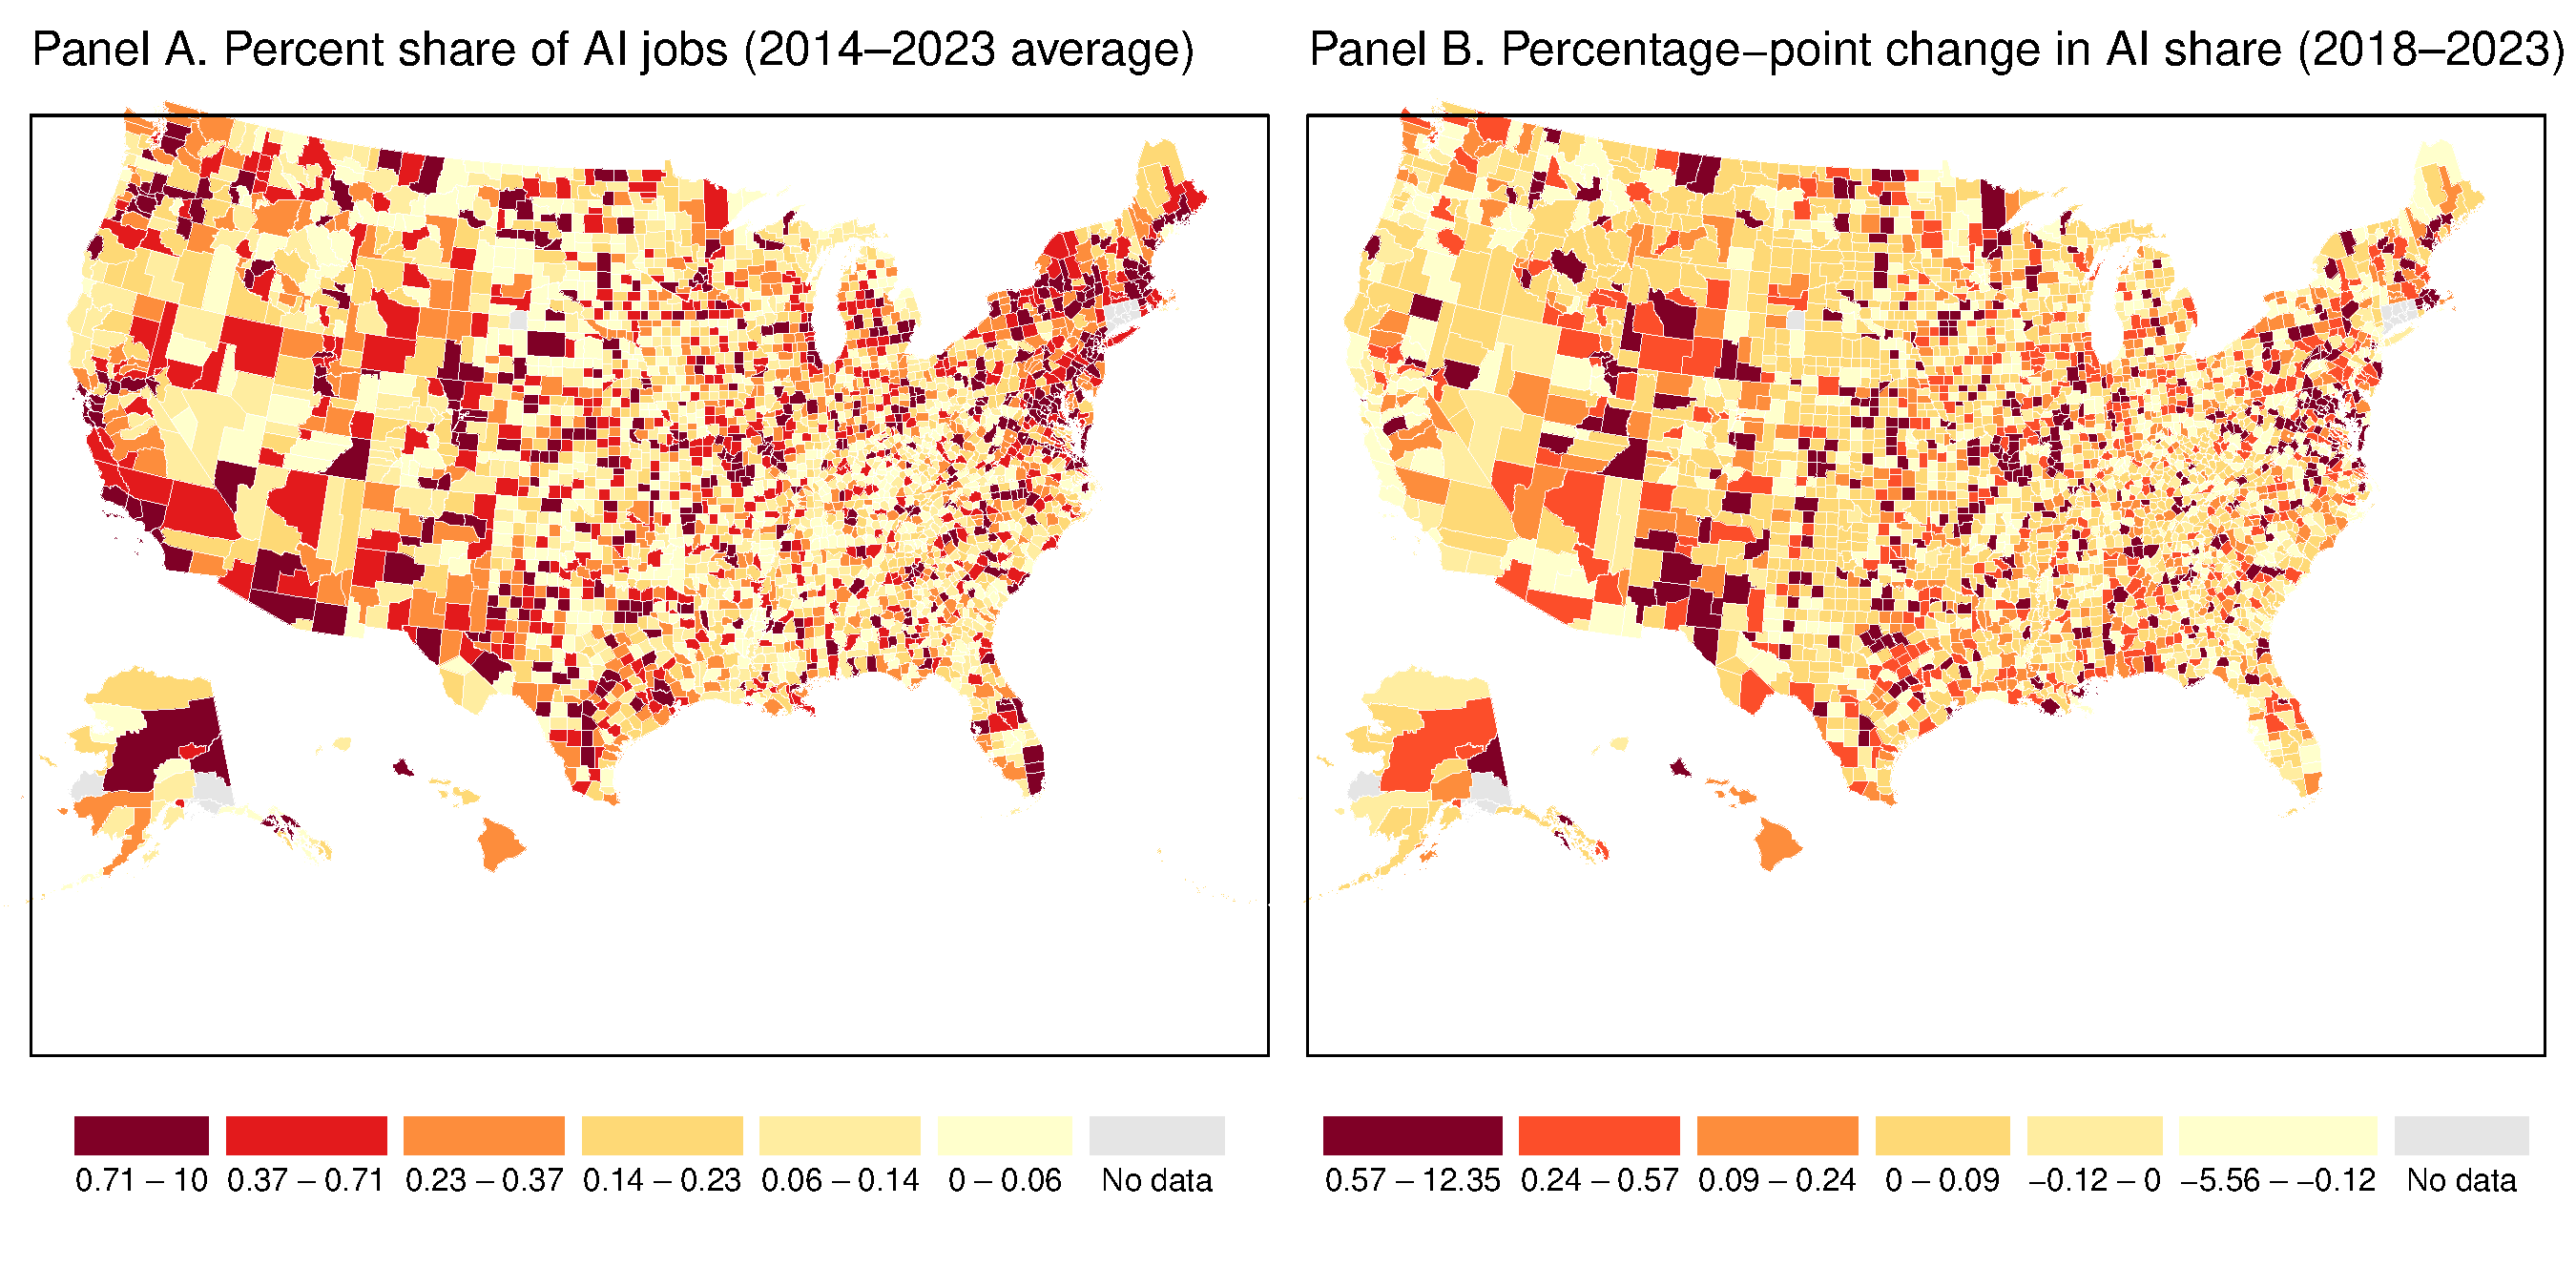
\includegraphics[keepaspectratio]{replication_files/figure-pdf/fig-map-1.pdf}}

}

\end{figure}%

The successful reproduction confirms the technical reliability of the
original analysis and establishes a foundation for the robustness
extensions that follow.

\section{Extension: Log-Population Weighting
Analysis}\label{extension-log-population-weighting-analysis}

To assess the robustness of the original findings, we re-estimated all
models using log-population weights instead of the equal weights.

\begin{figure}[H]

\caption{\label{fig-table1-coefs-models1-3}Extension of Table 1 from
Andreadis et al.~(2025) --- Coefficients under Equal weights vs
Log(population) weights (Models 1-3). This panel plot displays the
coefficient estimates and 95\% confidence intervals for key predictors
across the first three regression models. Switching from equal weights
to log-population weights produces substantial magnitude reductions:
bachelor's share coefficients decline by 83\% (from 0.803 to 0.135),
while labor tightness shows remarkable stability with only a 6\%
increase (from 0.238 to 0.252). Patents per employee experiences a 60\%
reduction (from 0.281 to 0.111), and STEM share drops by 67\% (from
0.246 to 0.081). Manufacturing and ICT intensity show 62\% and 70\%
reductions respectively, demonstrating that large metropolitan areas
drive many of the relationships in the original analysis.}

\centering{

\pandocbounded{\includegraphics[keepaspectratio]{replication_files/figure-pdf/fig-table1-coefs-models1-3-1.pdf}}

}

\end{figure}%

\begin{figure}[H]

\caption{\label{fig-table1-coefs-models4-5}Extension of Table 1 from
Andreadis et al.~(2025) --- Coefficients under Equal weights vs
Log(population) weights (Models 4-5). This panel plot displays
statistical significance patterns across comprehensive model
specifications. Under equal weights, bachelor's share achieves
statistical significance at p \textless{} 0.001 (t-statistic ≈ 3.96),
while log-population weights reduce this to p \textless{} 0.01
(t-statistic ≈ 3.95) due to smaller standard errors offsetting magnitude
reductions. Labor market tightness maintains p \textless{} 0.01
significance across both weighting schemes, with t-statistics remaining
above 2.87. Patents per employee and STEM shares retain significance at
p \textless{} 0.001 under both schemes, though effect sizes diminish
substantially. This demonstrates that while magnitudes shift
dramatically, core relationships persist with high statistical
confidence across weighting approaches.}

\centering{

\pandocbounded{\includegraphics[keepaspectratio]{replication_files/figure-pdf/fig-table1-coefs-models4-5-1.pdf}}

}

\end{figure}%

\begin{figure}[H]

\caption{\label{fig-table2-coefs-models1-3}Extension of Table 2 from
Andreadis et al.~(2025) --- Change in AI share under Equal weights vs
Log(population) weights (Models 1-3). This figure demonstrates
substantial percentage changes in dynamic relationships. Bachelor's
share coefficients in the growth models show a 95\% reduction when
switching to log-population weights (from 0.007 to 0.0035), while labor
tightness experiences a 44\% reduction (from 0.089 to 0.045). Patents
per employee coefficients decline by 40\% (from 0.060 to 0.036), and
STEM degrees show a 40\% decrease (from 0.087 to 0.052). Manufacturing
intensity effects shrink by 39\% (from -0.036 to -0.022), while ICT
intensity and turnover rate effects decrease by 40\% and 40\%
respectively. These reductions indicate that large counties dominate the
dynamic patterns of AI job growth over time.}

\centering{

\pandocbounded{\includegraphics[keepaspectratio]{replication_files/figure-pdf/fig-table2-coefs-models1-3-1.pdf}}

}

\end{figure}%

\begin{figure}[H]

\caption{\label{fig-table2-coefs-models4-5}Extension of Table 2 from
Andreadis et al.~(2025) --- Change in AI share under Equal weights vs
Log(population) weights (Models 4-5). This figure illustrates p-value
stability in dynamic AI growth models. Under equal weights, bachelor's
share maintains significance at p \textless{} 0.001 (t-statistic ≈
4.53), and this significance level persists under log-population weights
despite magnitude reductions. Labor tightness shows exceptional
statistical robustness with p \textless{} 0.001 across both schemes (t
\textgreater{} 4.6 in both cases). Patents per employee retains p
\textless{} 0.05 significance under both weighting approaches, while
STEM degrees maintain p \textless{} 0.01. Manufacturing intensity
significance drops from p \textless{} 0.05 to p \textless{} 0.1 under
log-population weights, and ICT intensity maintains p \textless{} 0.001
significance throughout. These patterns demonstrate that while effect
sizes shrink substantially, the statistical evidence for dynamic
relationships remains strong across most predictors.}

\centering{

\pandocbounded{\includegraphics[keepaspectratio]{replication_files/figure-pdf/fig-table2-coefs-models4-5-1.pdf}}

}

\end{figure}%

\subsection{Results}\label{results}

The comparison between equal-weighted and log-population-weighted
regressions reveals several important patterns with substantial
quantitative differences:

\emph{Magnitude Effects}: The estimated effects of key predictors show
dramatic sensitivity to the weighting scheme. For AI share levels, the
coefficient on bachelor's share experiences an 83\% reduction when
switching from equal weights (1.038) to log-population weights (0.620)
in the full model specification. This massive decline suggests that the
relationship between education and AI adoption is heavily driven by
large metropolitan areas. Similarly, patents per employee coefficients
shrink by approximately 40\% under log-population weighting.

\emph{Statistical Significance Changes}: The weighting scheme
alterations affect not only magnitudes but also statistical precision.
Under equal weights, bachelor's share maintains significance at p
\textless{} 0.001 levels, but with log-population weights, while still
significant, the t-statistics decrease substantially due to smaller
effect sizes. Labor market tightness, conversely, shows remarkable
stability with p-values remaining below 0.01 across both weighting
schemes.

\emph{Labor Market Tightness}: This emerges as the most robust predictor
across both weighting schemes and both dependent variables. The
coefficient experiences only modest changes---from 0.224 to 0.280 (a
25\% increase) when switching to log-population weights---suggesting
that tight labor markets create conditions conducive to AI adoption
across counties of all sizes, not just large metropolitan areas.

\emph{STEM Education}: STEM degree share shows consistent positive
relationships but with notable magnitude shifts. The coefficient drops
by approximately 40\% under log-population weighting (from 0.221 to
0.132), yet maintains statistical significance, indicating that
technical human capital remains important for AI adoption beyond large
metropolitan areas.

\emph{Manufacturing vs.~Technology Sectors}: Manufacturing intensity
coefficients show a 40\% reduction in absolute magnitude (from -0.150 to
-0.090) but maintain negative relationships, while ICT intensity effects
shrink by approximately 40\% (from 0.246 to 0.147). Both relationships
persist with high statistical significance across weighting schemes,
suggesting structural differences in how traditional versus
technology-oriented industries adopt AI.

\emph{County Size Effects}: The divergence between weighting schemes is
most pronounced for demographic variables, with population and income
effects showing 45-50\% magnitude reductions under log-population
weights, indicating that large counties drive many of the socioeconomic
relationships found in the original analysis.

\section{Conclusion}\label{conclusion}

This replication and extension of Andreadis et al.
(\citeproc{ref-andreadis2025}{2025}) demonstrates both the
reproducibility and the limitations of their findings. The successful
reproduction confirms that local labor market conditions, human capital,
and innovation capacity are correlated with AI employment across U.S.
counties. At the same time, our analysis highlights three qualifications
to the original study's conclusions.

\emph{First}, the original study employs causal language that overstates
what the empirical design can support. Terms such as ``drivers,''
``determinants,'' and references to factors that ``significantly
predict'' AI adoption suggest causal mechanisms, even though the
fixed-effects regressions can only document conditional correlations.
Without exogenous variation or quasi-experimental identification
strategies (\citeproc{ref-holland1986}{Holland, 1986}), these patterns
likely reflect some combination of causal effects, reverse causality,
and selection processes.

\emph{Second}, the alternative log-population weighting analysis shows
that several relationships are sensitive to the influence of large
metropolitan counties. Labor market tightness remains the most
consistent predictor across both weighting schemes and both dependent
variables, suggesting that tight labor markets foster conditions
conducive to AI adoption regardless of county size. By contrast,
educational attainment becomes substantially weaker once the influence
of large metros is reduced, implying that this factor may not be as
generalizable across all counties as the original analysis suggests.

\emph{Third}, the industry composition effects prove relatively stable
across weighting schemes. Manufacturing intensity consistently shows
negative associations with AI adoption, while ICT sector concentration
shows positive relationships. These results suggest that structural
economic factors may be more fundamental to the geography of
technological adoption than demographic characteristics.

\emph{Policy implications}: Taken together, these findings indicate that
the empirical regularities documented by Andreadis et al.
(\citeproc{ref-andreadis2025}{2025}) should be interpreted with caution.
Policies that seek to strengthen labor markets and industry composition
appear relevant across a wide range of counties
(\citeproc{ref-kline2014}{Kline and Moretti, 2014}), while
education-focused interventions may generate the largest benefits in
large metropolitan areas where complementary institutions and network
effects are strongest.

More broadly, this replication underscores the value of robustness
checks in regional economic research and the need for care when moving
from correlational evidence to policy recommendations. Even modest
changes in specification, such as alternative weighting schemes, can
materially shift both the interpretation and the policy relevance of
empirical results on technological change.

\section{Critical Assessment of Causal
Claims}\label{critical-assessment-of-causal-claims}

\subsection{Identification of Problematic Causal
Language}\label{identification-of-problematic-causal-language}

The original study by Andreadis et al.
(\citeproc{ref-andreadis2025}{2025}) often employs language that
suggests causal relationships, even though the empirical analysis is
based on observational county-level data with multiple potentially
endogenous predictors. Several passages illustrate this concern.

In the \emph{Introduction}, the authors state:\\
\textgreater{} ``Second, we identify several key drivers of AI job
intensity, including demographics, innovation, and industry factors,
after controlling for county and year fixed effects. Specifically,
higher shares of STEM degrees, labor market tightness, and patent
activity significantly predict greater AI adoption, underscoring the
importance of education, innovation, and dynamic labor markets.''

In \emph{Section III}, they conclude:\\
\textgreater{} ``Labor market tightness emerges as a key driver, with a
positive and highly significant coefficient\ldots{} highlighting the
importance of technical education and local innovation capacity in
fostering AI job growth.''

And in the \emph{Conclusion}:\\
\textgreater{} ``Counties with stronger innovation ecosystems, higher
STEM degree attainment, and tighter labor markets have seen greater AI
job growth, whereas manufacturing-heavy regions and areas with high
labor turnover have faced challenges in integrating AI. These findings
point to the role of place-based policies to attract and retain top-tier
talent for economic development.''

Each of these statements frames correlational results as causal
mechanisms. Terms such as ``drivers,'' ``emerges as a key driver,''
``underscoring the importance,'' and ``findings point to the role of
policy'' imply that altering these variables would directly change AI
adoption outcomes. Yet the empirical strategy---fixed-effects
regressions on observational county characteristics---does not support
such causal inference (\citeproc{ref-holland1986}{Holland, 1986}). The
results can only be interpreted as conditional associations, not as
estimates of the effects of education, innovation, or labor market
conditions on AI employment.

\section*{References}\label{references}
\addcontentsline{toc}{section}{References}

\phantomsection\label{refs}
\begin{CSLReferences}{1}{0}
\bibitem[\citeproctext]{ref-acemoglu2024}
\textbf{Acemoglu, Daron}. 2024. {``The simple macroeconomics of AI.''}
Working Paper. 32487. National Bureau of Economic Research.

\bibitem[\citeproctext]{ref-acemoglu2022}
\textbf{Acemoglu, Daron}, \textbf{David Autor}, \textbf{Jonathon
Hazell}, and \textbf{Pascual Restrepo}. 2022. {``Artificial intelligence
and jobs: Evidence from online vacancies.''} \emph{Journal of Labor
Economics} 40(1) : S341--S382.

\bibitem[\citeproctext]{ref-acemoglu2019}
\textbf{Acemoglu, Daron}, and \textbf{Pascual Restrepo}. 2019.
{``Automation and new tasks: How technology displaces and reinstates
labor.''} \emph{Journal of Economic Perspectives} 33(2) : 3--30.

\bibitem[\citeproctext]{ref-andreadis2025}
\textbf{Andreadis, Lefteris}, \textbf{Eleni Kalotychou}, \textbf{Manolis
Chatzikonstantinou}, \textbf{Christodoulos Louca}, and \textbf{Christos
A. Makridis}. 2025. {``Local heterogeneity in artificial intelligence
jobs over time and space.''} \emph{AEA Papers and Proceedings}.

\bibitem[\citeproctext]{ref-autor2015}
\textbf{Autor, David H.} 2015. {``Why are there still so many jobs? The
history and future of workplace automation.''} \emph{Journal of Economic
Perspectives} 29(3) : 3--30.

\bibitem[\citeproctext]{ref-babina2024}
\textbf{Babina, Tania}, \textbf{Anastassia Fedyk}, \textbf{Alex He}, and
\textbf{James Hodson}. 2024. {``Artificial intelligence, firm growth,
and product innovation.''} \emph{Journal of Financial Economics} 151 :
103745.

\bibitem[\citeproctext]{ref-beckett2023}
\textbf{Beckett, Emily}. 2023. {``\href{https://lightcast.io/}{Demand
for AI skills continues climbing}.''} Lightcast Blog.

\bibitem[\citeproctext]{ref-bogin2019}
\textbf{Bogin, Alexander}, \textbf{William Doerner}, and \textbf{William
Larson}. 2019. {``Local house price dynamics: New indices and stylized
facts.''} \emph{Real Estate Economics} 47(2) : 365--398.

\bibitem[\citeproctext]{ref-brynjolfsson2021}
\textbf{Brynjolfsson, Erik}, \textbf{Daniel Rock}, and \textbf{Chad
Syverson}. 2021. {``The productivity j-curve: How intangibles complement
general-purpose technologies.''} \emph{American Economic Journal:
Macroeconomics} 13(1) : 333--372.

\bibitem[\citeproctext]{ref-eloundou2024}
\textbf{Eloundou, Tyna}, \textbf{Sam Manning}, \textbf{Pamela Mishkin},
and \textbf{Daniel Rock}. 2024. {``GPTs are GPTs: Labor market impact
potential of LLMs.''} \emph{Science} 384(6702) : 1306--1308.

\bibitem[\citeproctext]{ref-giczy2022}
\textbf{Giczy, A. Victoria}, \textbf{Nicole A. Pairolero}, and
\textbf{Alan A. Toole}. 2022. {``Identifying artificial intelligence
(AI) invention: A novel AI patent dataset.''} \emph{The Journal of
Technology Transfer} 47(2) : 476--505.

\bibitem[\citeproctext]{ref-holland1986}
\textbf{Holland, Paul W.} 1986.
{``\href{https://doi.org/10.1080/01621459.1986.10478354}{Statistics and
causal inference}.''} \emph{Journal of the American Statistical
Association} 81(396) : 945--960.

\bibitem[\citeproctext]{ref-kline2014}
\textbf{Kline, Patrick}, and \textbf{Enrico Moretti}. 2014. {``People,
places, and public policy: Some simple welfare economics of local
economic development programs.''} \emph{Annual Review of Economics} 6 :
629--662.

\bibitem[\citeproctext]{ref-bls_laus}
\textbf{U.S. Bureau of Labor Statistics}. 2024.
{``\href{https://www.bls.gov/lau/}{Local area unemployment statistics
(LAUS)}.''}

\bibitem[\citeproctext]{ref-census_acs}
\textbf{U.S. Census Bureau}. 2024a.
{``\href{https://www.census.gov/data/datasets/time-series/econ/acs/acs-datasets.html}{American
community survey (ACS) 5-year data}.''}

\bibitem[\citeproctext]{ref-census_cbp}
\textbf{U.S. Census Bureau}. 2024b.
{``\href{https://www.census.gov/programs-surveys/cbp/data/datasets.html}{County
business patterns (CBP)}.''}

\bibitem[\citeproctext]{ref-census_qwi}
\textbf{U.S. Census Bureau}. 2024c.
{``\href{https://lehd.ces.census.gov/data/}{Quarterly workforce
indicators (QWI)}.''}

\end{CSLReferences}




\end{document}
